\section{Reock}\label{sec:reock}
Let $\mathrm{circ}(\Omega)$ denote the \textit{smallest bounding
circle} (smallest bounding \textit{cap} on the sphere) of a region
$\Omega$.  Then the \textit{Reock score} of $\Omega$ is 

$$\mathrm{Reock}(\Omega)=
\frac{\mathrm{area}(\Omega)}{\mathrm{area}(\mathrm{circ}(\Omega))}.$$
\begin{lemma}
  Let $\vphi:S^2\to\R^2$ be a map projection preserving the 
  ordering of Reock scores. Then, after 
  possibly restricting its domain, $\vphi$ must
  \begin{enumerate}
    \item Send spherical caps to Euclidean balls
    \item Preserve area equality
  \end{enumerate}
\end{lemma}
\begin{proof}
  Since $\vphi$ preserves the ordering of Reock scores, it must 
  send maximizers of this score on the sphere to corresponding 
  maximizers in the plane, giving the first condition.

  Next, let $\kappa$ be a cap on the sphere, and let 
  $X,Y\subset \kappa$ be two sets properly contained in 
  $\kappa$ of equal area. Then:
  \begin{align*}
    \mathrm{Reock}(\kappa\ssm X) 
    = 1-\frac{\mathrm{Area}(X)}{\mathrm{Area}(\kappa)} 
    = 1-\frac{\mathrm{Area}(Y)}{\mathrm{Area}(\kappa)}
    = \mathrm{Reock}(\kappa\ssm Y)
  \end{align*}
  Note that $\kappa$ is sent to a circle in the plane, so 
  the minimal bounding circle of $\vphi(\kappa)$ is itself. Thus, 
  since $\vphi$ preserves equality of Reock scores,
  \begin{align*}
    1-\frac{\mathrm{Area}(\vphi(X))}{\mathrm{Area}(\vphi(\kappa))} 
    = \mathrm{Reock}(\vphi(\kappa\ssm X)) 
    = \mathrm{Reock}(\kappa\ssm Y)
    = 1-\frac{\mathrm{Area}(\vphi(Y))}{\mathrm{Area}(\vphi(\kappa))}
  \end{align*}
  Meaning that $\mathrm{Area}(\vphi(X)) = \mathrm{Area}(\vphi(Y))$. 
  Thus, restricting $\vphi$ to $\kappa$, we get that 
  $\vphi$ preserves area equality.
\end{proof}
\begin{remark}
  The above proof also holds for $\vphi^{-1}$
\end{remark}
\begin{lemma}
  Let $V\subset S^2$ and $U\subset \R^2$ be open. There does not exist a 
  diffeomorphism $\vphi:U\to V$ which sends spherical caps 
  to Euclidean balls and preserves area equality.
\end{lemma}
\begin{proof}
  We consider the following configuration of equal-radius circles in $U$:
  \begin{center}
    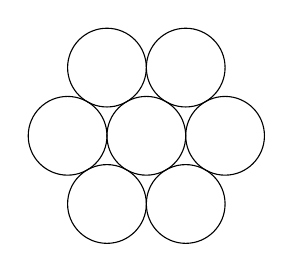
\begin{tikzpicture}
      \draw (0,0) circle (0.5);
      \draw (1,0) circle (0.5);
      \draw ({cos(60)},{sin(60)}) circle (0.5);
      \draw ({cos(120)},{sin(120)}) circle (0.5);
      \draw ({cos(180)},{sin(180)}) circle (0.5);
      \draw ({cos(240)},{sin(240)}) circle (0.5);
      \draw ({cos(300)},{sin(300)}) circle (0.5);
    \end{tikzpicture}
  \end{center}
  Under $\vphi$, they must be sent to an equivalent configuration 
  of caps on the sphere of equal area. Since the radius 
  of a spherical cap is uniquelty determined by its area, it follows 
  that each of these circles is sent to a cap of equal radius. Thus, 
  the midpoints of these caps form six equallateral triangles 
  in $S^2$ meeting at a point, which cannot happen, as each triangle 
  has angles larger than $\frac{\pi}{3}$.
\end{proof}
Piecing the above lemmas together yields:
\begin{theorem}
  Let $U\subset S^2$ be some open region, and let 
  $\vphi:U\to \R^2$ be a map projection. Then 
  $\vphi$ does not preserve the ordering of Reock scores.
\end{theorem}
